% Since \input doesn't like preambles, only uncomment next line if you're editing this TeX, don't forget the \end{document}! 
%\documentclass{article}\usepackage[utf8]{inputenc} % allows for non-ASCII input characters like ä
\usepackage[x11names]{xcolor}% Color extensions, load first
\usepackage[margin=1in]{geometry} % Formatting on page
\usepackage{array} % better arrays
\usepackage{amsmath} % Math symbols and formats
    \numberwithin{equation}{section} % amsmath command that renews equation counter in each section\
\usepackage{amsthm}   
\usepackage{amssymb}
\usepackage[backend=bibtex]{biblatex} % bibliography
\usepackage{bm} % bold, even for greek letters
\usepackage{enumitem} % Enumerating things
\usepackage{esint} % better double and triple Integrals
\usepackage{etoc} % super powerful table of contents
\usepackage{fancyhdr} % Headers
    \pagestyle{fancy}
\usepackage{gensymb} % more symbols
\usepackage{physics} % easier commands for physics things
\usepackage{relsize}  % allows for larger/smaller math 
\usepackage{textcomp} % Gets rid of perthousand error
\usepackage{upquote}  % fixes quotes in verbatim environment
\usepackage{verbatim} % Allows for comment environment
\usepackage{tikz} % pictures and drawings
    \usetikzlibrary{calc}
    \usetikzlibrary{3d}
    %\usetikzlibrary{external}
    %\tikzexternalize
    %\tikzsetexternalprefix{figures/}
\usepackage{pgfplots} % plots and graphics
    \pgfplotsset{compat=newest} % or use compat=1.6 
\usepackage{graphicx} % plots and graphics
\usepackage{xparse} % Better commands
\usepackage[hidelinks]{hyperref}% References--THIS GOES LAST
\usepackage[utf8]{inputenc} % allows for non-ASCII characters
\usepackage[x11names]{xcolor}    % Color extensions
\usepackage[margin=1in]{geometry} % Formatting on page
\usepackage{array} % big arrays
\usepackage{amsmath} % Math symbols
\usepackage{amsthm}   
\usepackage{amssymb}
\usepackage[backend=bibtex]{biblatex} % bibliography
\usepackage{bm} % bold for greek letters
\usepackage{cancel}
\usepackage[format=hang]{caption}
\usepackage{enumitem} % Enumerating things
\usepackage{esint} % better double and triple Integrals
\usepackage{etoc}
\usepackage{fancyhdr} % Headers
    \pagestyle{fancy}
\usepackage{float}
\usepackage{gensymb}
\usepackage{physics} % easier commands for physics things
\usepackage{relsize}  % allows for larger/smaller math 
\usepackage{textcomp} % Gets rid of perthousand error
\usepackage{upquote}  % fixes quotes in verbatim environment
\usepackage{verbatim} % Allows for comment environment
\usepackage{tikz} % pictures
	\usetikzlibrary{calc}
	\usetikzlibrary{decorations.markings}
	\usetikzlibrary{3d}
	\usetikzlibrary{intersections}
\usepackage{pgfplots} % plots and graphics
	\pgfplotsset{compat=newest} % or use compat=1.6
	\usepgfplotslibrary{fillbetween}
\usepackage{graphicx} % plots and graphics
\usepackage{wrapfig}
\usepackage{xparse} % Better commands
\usepackage[hidelinks]{hyperref}% References--THIS GOES LAST

% Packages that this breaks without: amsmath, gensymb, physics, hyperref, xcolor, xparse, and possibly others
\numberwithin{equation}{section} % amsmath command that renews equation counter in each section\
\def\ints{\int_\mathcal{S}} % Surface integral
\def\intv{\int_\mathcal{V}} % Volume integral with V subscript
\def\intall{\int_{-\infty}^{\infty}} % Integral over all space
\def\iintall{\iint_{\rm All Space}} % Integral over all space
\def\iiintall{\iiint_{\rm All Space}} % Integral over all space
\def\ik{4\pi\epsilon_0} % Inverse k for EM
\def\lap{\mathcal{L}}
\def\answerline{ % double horizontal line placed 0.5 cm below text, space between lines is 0.07 cm, then 0.75 cm of space 
	\vspace{0.5 cm}
	\hrule
	\vspace{0.07 cm}
	\hrule
	\vspace{0.75 cm}\noindent} % don't indent text after the line
\NewDocumentCommand\length{O{3pt}}{\setlength\jot{#1}} % for align vertical spacing, there's probably a better way to do this locally
\NewDocumentCommand\ft{s O{n} O{L}}{ % I dont want to write \sin(stuff) \cos(stuff) every time in fourier transforms (ft)
    \IfBooleanTF{#1}{
        \sin(\frac{#2 \pi}{#3}x)
    }{
        \cos(\frac{#2 \pi}{#3}x)
    }
}

\NewDocumentCommand\dl{s}{\IfBooleanTF{#1}{}{\cdot} d\mathbf{l}} % quicker curve integral dl, if no star, it also makes the dot 
\NewDocumentCommand\da{s}{\IfBooleanTF{#1}{}{\cdot} d\mathbf{a}} % quicker surface integral da, if no star, it also makes the dot 
\NewDocumentCommand\oo{O{1} m} {\frac{#1}{#2}}   % reciprocal- 'one over', option to make it a regular fraction because oo is still quicker to type.
\NewDocumentCommand\thetitle{m O{}}{ \title{ \hypertarget{top}{\textbf{#1}} \\ \large {#2} } } %Bold title that is a hypertarget, optional bolded subtitle that's scaled properly 

\NewDocumentCommand \e {s m}{ % basis vector command
	\IfBooleanTF{#1} % \e{x} for x hat notation, \e*{x} for e_x notation
	{\mathbf{\hat{e}_{#2}}}
	{\bm{\hat{#2}}}} % from package bm, more powerful than \mathbf} 
\NewDocumentCommand \parametric {m}{ %command for getting boundary conditions with a "{" on the left
    \left\{ 
	\begin{gathered}
		\begin{matrix}
			#1
    		\end{matrix}
	\end{gathered}
	 \right.}
\NewDocumentCommand \der {s O{} m g}{ % custom derivative command
     \IfBooleanTF{#1} % if \der*, #1 is true, euler notation used, if \der , #1 is false, d/dx is used 
    {\IfNoValueTF{#4}  % g returns -NoValue- if no argument (read below)
        {\mathrm{D}_{#3}^{#2}}  % g is included so \der{x} and \der{f}{x} both have x in the denominator
        {\mathrm{D}_{#4}^{#2}#3}
            }
    {\IfNoValueTF{#4}
        {\frac{\mathrm{d}^{#2}}{\mathrm{d} #3^{#2}}}
        {\frac{\mathrm{d}^{#2} #3}{\mathrm{d} #4^{#2}}}
	}}    
\NewDocumentCommand \pder {s O{} m g d[]}{ % custom partial derivative command, allows for euler notation if starred, added d[] entry for parenthesis around derivative for quantities that are held constant 
	\IfBooleanTF{#1} % Star for euler notation
	   {\IfNoValueTF{#4} % Logic with #4 is so first argument gets put in denomenator if there is only one ( like \pder{x} ), but if there are two arguments (#4 is second argument) then the second argument is put in denominator \pder{f}{x}
		   {\partial_{#3}^{#2}}
		   {\partial_{#4}^{#2}#3}
			   }
	   {\IfNoValueTF{#5} % #5 is what is held constant
		   {\IfNoValueTF{#4}
			   {\frac{\partial^{#2}}{\partial #3^{#2}}}
			   {\frac{\partial^{#2} #3}{\partial #4^{#2}}}}
		   {{\IfNoValueTF{#4} 
			   {\left(\frac{\partial^{#2}}{\partial #3^{#2}}\right)_{\!#5}\!\!} % \! is thin negative space
			   {\left(\frac{\partial^{#2} #3}{\partial #4^{#2}}\right)_{\!#5}\!\!}}}
			   }} 
                
\NewDocumentCommand \header {m m m}{
	\fancyhead[L]{#1} 
	\fancyhead[C]{\hyperlink{top}{ \textbf{#2} }}
	\fancyhead[R]{#3}
	\fancyfoot[C]{--\thepage--}
	\pagestyle{fancy}
	\setlength\headheight{17pt}}
    
\NewDocumentCommand{\coloredanswer}{O{LavenderBlush2} m}{ % makes coloredbox with pretty color
	\mathchoice
	{\colorbox{#1}{$\displaystyle #2$}}
	{\colorbox{#1}{$\textstyle #2$}}
	{}
	{}}

\newcounter{probcount} % new counter for problem numbers, starts at 0 by default
\NewDocumentEnvironment{ problem } {O{} +b} %Problem environment for homework, autocounts numbers, behaves like a section and can get listed (and hyperlinked) in the toc. 
	{\addtocounter{probcount}{1} % increase counter at the beginning of every problem
	 \phantomsection % invisible page marker for hyperref
	 \addcontentsline{toc}{subsection}{Problem \theprobcount~{\it#1}} % add "Problem \theprobcount. \textit{#1}" to table of contents (toc) as if it were a subsection
	 \begin{trivlist} % begin unmarked ("trivial") list
	 \item {\bf Problem \theprobcount} {\it#1} % print Problem with the counter and optional text 
	 \item #2  % +b is for inputs that are long
	 \end{trivlist} % end list
	}{} % don't do anything then "problem" environment ends, irrelevant because trivlist is already ended
	
\def\UM{\colorbox{blue}{\textcolor{Gold1}{\textbf{University of Michigan}}}} % School Pride
\def\EC{\href{https://github.com/CarpenterEvan/PhysicsReview}{\(\mathbb{E}\textsc{van}~\mathbb{C}\textsc{arpenter}\)}}
\endinput\begin{document}
\section{Special Functions}  
    Special functions functions that are defined to have established names and properties because of their importance. Simple examples of special functions are the {\bf sin and log} functions. Some of them are unintuitive, and the notation is often weird, but analysis becomes easier if you use them. 
    \subsection{Bessel Functions}
        Bessel functions are defined to be solutions to Bessel's differential equation:
        \begin{gather}
            x^2y''(x)+xy'(x)+\qty(\lambda x^2-n^2)y(x)=0\quad\parametric{ n\in\mathbb{N}\\\lambda>0\\x\geq0}
            \\
            y(x)=c_1J_n(\sqrt{\lambda}x)
        \end{gather}
        Where $J_n$ is a Bessel function of the first kind. 
    \subsection{Dirac Delta Function}
        Given that the product $f(x)\delta(x)$ is zero everywhere except at x = 0:
        \begin{align*}
            \delta(x)\equiv\parametric{
            \infty & x=0
            \\
            0 & x\neq 0
            \\[0.25 cm]
            \int_{-\infty}^\infty \delta(x) dx &= 1}
        \end{align*}
        As a result of the definition:
        \begin{align*}
            \intall f(x) \delta(x-a) dx 
            &= f(a)
        \end{align*}
        \subsubsection*{Three-dimensional Dirac Delta Function}
            The Dirac Delta Function picks out the value of the function f at the location of the space in question.
            \begin{align*}
                {\delta}^3(r) &= \delta(x) \delta(y) \delta(z)
            \end{align*}
            \begin{align*}
                \intall f(r) {\delta}^3(r-a) dV &= f(a)
            \end{align*}
            A useful version of this, re-casted for use in electrodynamics:
            \begin{align*}
                \div\qty(\frac{\e{r}}{{r}^2}) &= 4 \pi {\delta}^3(\vb{r})
            \end{align*}\newpage
    \subsection{Error Function}
    \subsection{Gamma Function}
    \subsection{Hermite Polynomials}
    \subsection{Laguerre Polynomials}
    \subsection{Legendre Polynomials}
        They are solutions to \textit{Legendre's Differential Equation}:
        %\tikzsetnextfilename{legendre}
        \begin{equation}
            \qty(1-x^2)y''(x)-2xy'(x)+n(n+1)y(x)=0\quad\parametric{n\in\mathbb{N}\\-1\leq x\leq 1}
        \end{equation}
        They can also be generated by the Rodriguez formula, a much easier way to find Legendre Polynomials:\cite{pinsky_2011}
        \begin{equation}
            P_n(x)=\oo{2^nn!}\der[n]{x}\qty[\qty(x^2-1)^n]
        \end{equation}
        \begin{figure}[h!]
            \centering
            \begin{tikzpicture}[scale=1.25]
                \begin{axis}[range=-1:1,domain=-1:1, thick, legend pos= outer north east]
                    \addplot[samples=2]{1};
                    \addplot[samples=10, blue]{x};
                    \addplot[samples=20, purple]{(3*x^2-1)/2};
                            \addplot[samples=40, yellow!50!orange]{(5*x^3-3*x)/2};
                            \legend{1, 
                            $x$,
                            $\oo{2}\qty(3x^2-1)$,
                            $\oo{2}\qty(5x^3-3x)$}
                \end{axis}
            \end{tikzpicture}
            \caption{The First Five Legendre Polynomials ($n=0,1,2,3,4$)}
            \label{fig:legendre_graph}
        \end{figure}
%\end{document}